\HeadingLevelB{Software Attestation Overview}
\label{sec:generic_software_attestation}

The security of systems that employ trusted processors hinges on
\textit{software attestation}. The software running inside an \textit{isolated
container} established by trusted hardware can ask the hardware to
sign~(\S~\ref{sec:integrity_crypto}) a small piece of \textit{attestation
data}, producing an \textit{attestation signature}. Asides from the attestation
data, the signed message includes a \textit{measurement} that uniquely
identifies the software inside the container. Therefore, an attestation
signature can be used to convince a \textit{verifier} that the attestation data
was produced by a specific piece of software, which is hosted inside a
container that is isolated by trusted hardware from outside interference.

Each hardware platform discussed in this section uses a slightly different
software attestation scheme. Platforms differ by the amount of software that
executes inside an isolated container, by the isolation guarantees provided to
the software inside a container, and by the process used to obtain a
container's measurement. The threat model and security properties of each
trusted hardware platform follow directly from the design choices outlined
above, so a good understanding of attestation is a prerequisite to discussing
the differences between existing platforms.


\HeadingLevelC{Authenticated Key Agreement}

Software attestation can be combined with a key agreement
protocol~(\S~\ref{sec:key_agreement}), as software attestation provides the
authentication required by the key agreement protocol. The resulting protocol can
assure a verifier that it has established a shared secret with a specific piece
of software, hosted inside an isolated container created by trusted hardware.
The next paragraph outlines the augmented protocol, using Diffie-Hellman Key
Exchange~(DKE)~\cite{diffie1976keyexchange} as an example of the key exchange
protocol.

The verifier starts executing the key exchange protocol, and sends the first
message, $g^{A}$, to the software inside the secure container. The software
inside the container produces the second key exchange message, $g^{B}$, and
asks the trusted hardware to attest the cryptographic hash of both key exchange
messages, $h(g^{A} || g^{B})$. The verifier receives the second key exchange
and attestation signature, and authenticates the software inside the secure
container by checking all the signatures along the \textit{attestation chain}
of trust shown in Figure~\ref{fig:generic_attestation_chain}.

\begin{figure}[hbt]
  \centering
  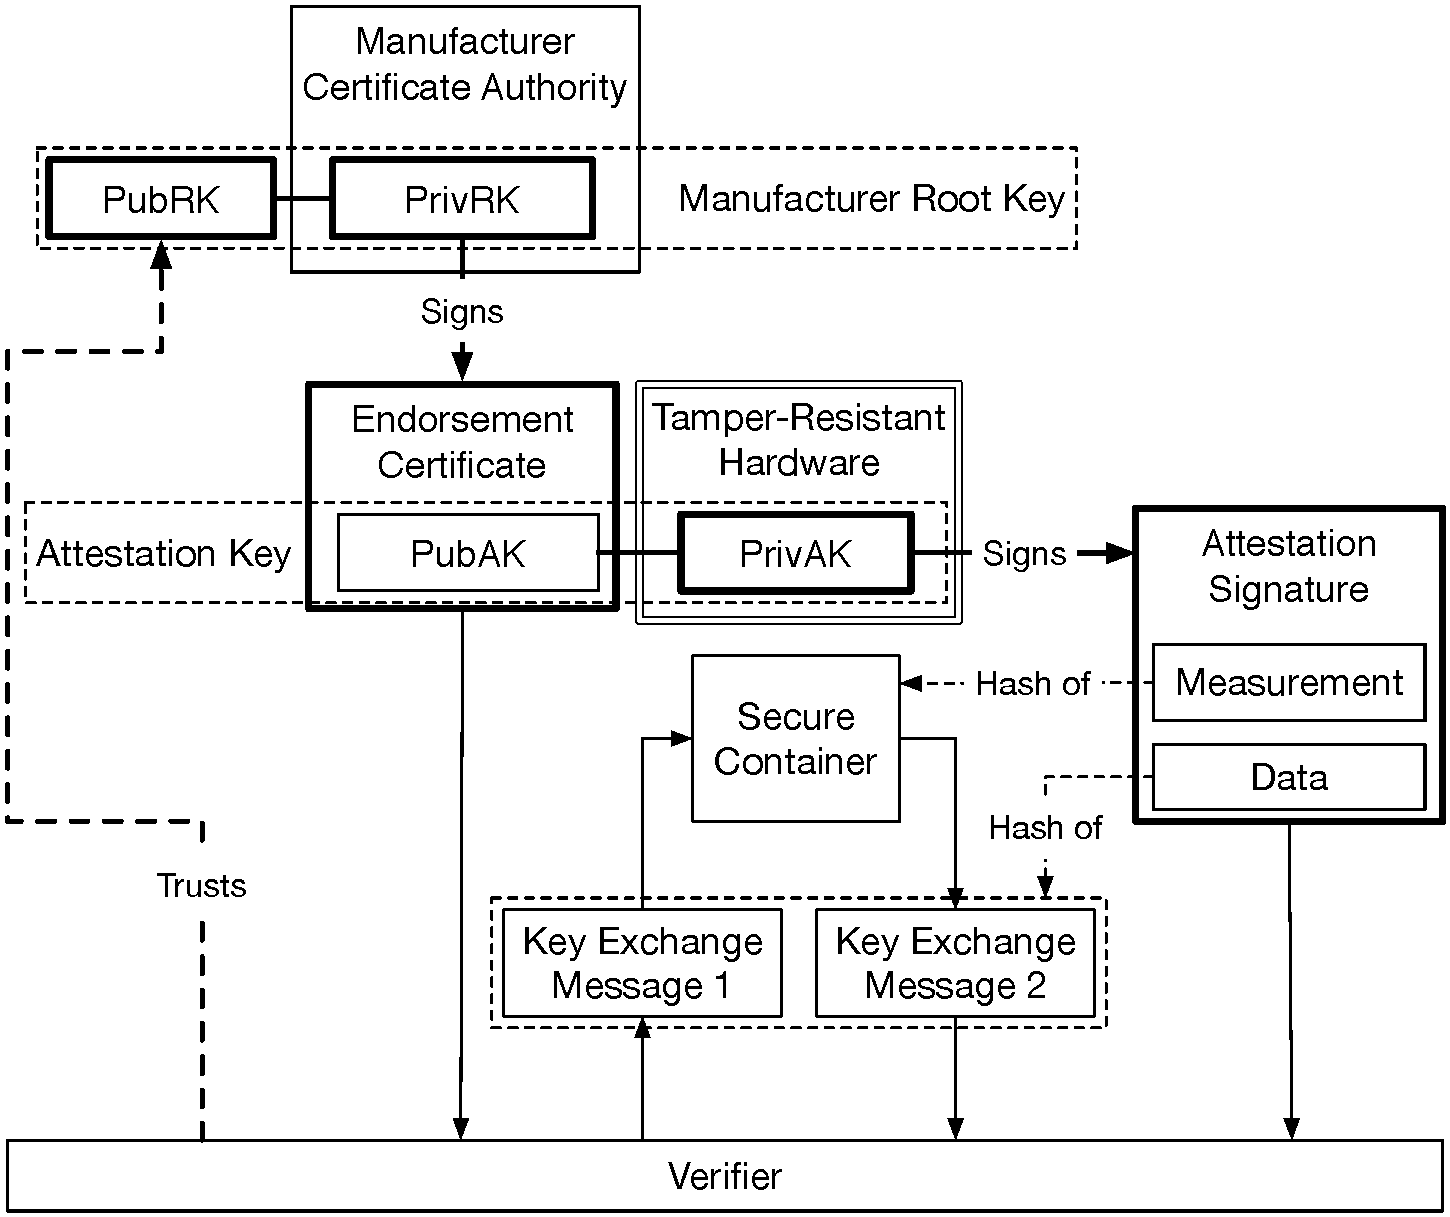
\includegraphics[width=85mm]{figures/generic_attestation_chain.pdf}
  \caption{
    The chain of trust in software attestation. The root of trust is a
    manufacturer key, which produces an endorsement certificate for the secure
    processor's attestation key. The processor uses the attestation key to
    produce the attestation signature, which contains a cryptographic hash of
    the container and a message produced by the software inside the container.
  }
  \label{fig:generic_attestation_chain}
\end{figure}

The chain of trust used in software attestation is rooted at a signing key
owned by the hardware manufacturer, which must be trusted by the verifier. The
manufacturer acts as a Certificate Authority (CA, \S~\ref{sec:certificates}),
and provisions each secure processor that it produces with a unique
\textit{attestation key}, which is used to produce
\textit{attestation signatures}. The manufacturer also
issues an \textit{endorsement certificate} for each secure processor's
attestation key. The certificate indicates that the key is meant to be used for
software attestation. The certification policy generally states that, at the
very least, the private part of the attestation key be stored in
tamper-resistant hardware, and only be used to produce attestation signatures.

A secure processor identifies each isolated container by storing a
cryptographic hash of the code and data loaded inside the container. When the
processor is asked to sign a piece of attestation data, it uses the
cryptographic hash associated with the container as the measurement in the
attestation signature. After a verifier validates the processor's attestation
key using its endorsement certificate, the verifier ensures that the signature
is valid, and that the measurement in the signature belongs to the software with
which it expects to communicate. Having checked all the links in the
attestation chain, the verifier has authenticated the other party in the key
exchange, and is assured that it now shares a secret with the software that it
expects, running in an isolated container on hardware that it trusts.


\HeadingLevelC{The Role of Software Measurement}
\label{sec:generic_measurement}

The measurement that identifies the software inside a secure container is
always computed using a secure hashing
algorithm~(\S~\ref{sec:integrity_crypto}). Trusted hardware designs differ in
their secure hash function choices, and in the data provided to the hash
function. However, all the designs share the principle that each step taken to
build a secure container contributes data to its measurement hash.

The philosophy behind software attestation is that the computer's owner can
load any software she wishes in a secure container. However, the computer owner
is assumed to have an incentive to participate in a distributed system where
the secure container she built is authenticated via software attestation.
Without the requirement to undergo software attestation, the computer owner can
build any container without constraints, which would make it impossible to
reason about the security properties of the software inside the container.

By the argument above, a trusted hardware design based on software attestation
must assume that each container is involved in software attestation, and that
the remote party will refuse to interact with a container whose reported
measurement does not match the expected value set by the distributed system's
author.

For example, a cloud infrastructure provider should be able to use the secure
containers provided by trusted hardware to run any software she wishes on her
computers. However, the provider makes money by renting her infrastructure to
customers. If security savvy customers are only willing to rent containers
provided by trusted hardware, and use software attestation to authenticate the
containers that they use, the cloud provider will have a strong financial
incentive to build the customers' containers according to their specifications,
so that the containers pass the software attestation.

A container's measurement is computed using a secure hashing algorithm, so the
only method of building a container that matches an expected measurement is to
follow the exact sequence of steps specified by the distributed system's
author. The cryptographic properties of the secure hash function guarantee that
if the computer's owner strays in any way from the prescribed sequence of
steps, the measurement of the created container will not match the value
expected by the distributed system's author, so the container will be rejected
by the software attestation process.

Therefore, it makes sense to state that a trusted hardware design's measurement
scheme guarantees that a property has a certain value in a secure container.
The precise meaning of the phrase is that the property's value determines the
the data used to compute the container's measurement, so an expected
measurement hash effectively specifies an expected value for the property. The
correct use of software attestation in a distributed system will cause all
containers that are allowed to participate in the system to have the desired
value for the given property.

For example, the measuring scheme used by trusted hardware designed for cloud
infrastructure should guarantee that the container's memory was initialized
using the contents desired by the customer. This contents is often referred to
as an image.
